\subparagraph{Задание 4.9}

\textbf{Условие}:
Выполнить 2 прохода цикла по F7, контролируя значения регистров. Для этого необходимо открыть окно CPU (View->CPU). Какие регистры изменяются в цикле?

Привести результаты выполнения данного фрагмента программы в отчете в виде таблицы: пример таблица~\ref{tab:task_4_9} (стр.~\pageref{tab:task_4_9}).

\begin{table}[!ht]
    \centering
    \caption{Пример таблицы для задания}
    \label{tab:task_4_9}
    \begin{tabular}{|c|c|c|c|c|c|} 
        \hline
        № шага  & IP  & AX  & BX  & CX  & DX  \\ \hline
        \hline
        1       &     &     &     &     &     \\ \hline
        2       &     &     &     &     &     \\ \hline
        ...     &     &     &     &     &     \\ \hline
    \end{tabular}
\end{table}

Объяснить в отчете изменения регистров

\textbf{Решение}:

В Turbo Debugger жмем F10. Попадаем в Меню. Жмем два раза вправо. Выбираем пунтк View. Enter. Жмем 7 раз вниз. Enter. Вводим для поиска метку NextLoop. Рисунок~\ref{fig:task_4_9__View_Watches} (стр.~\pageref{fig:task_4_9__View_Watches}).

Жмем Alt+F9. Вводим NextLoop. Enter. Рисунок~\ref{fig:task_4_9__Alt_F9} (стр.~\pageref{fig:task_4_9__Alt_F9}).

Перешли к метке. Результат на рисуноке~\ref{fig:task_4_9__Alt_F9_result} (стр.~\pageref{fig:task_4_9__Alt_F9_result}).

\begin{figure}[!htp]
    \centering
    \begin{minipage}{0.32\textwidth}
        \centering
        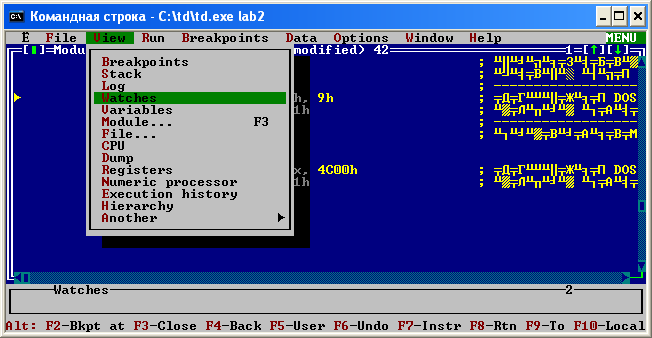
\includegraphics[width=.99\linewidth]
            {../_INCLUDES/task-4-9/td-View-Watches.png}
        \caption{\textbf{View}>\textbf{Wathes}}
        \label{fig:task_4_9__View_Watches}
    \end{minipage}
    \begin {minipage}{0.32\textwidth}
        \centering
        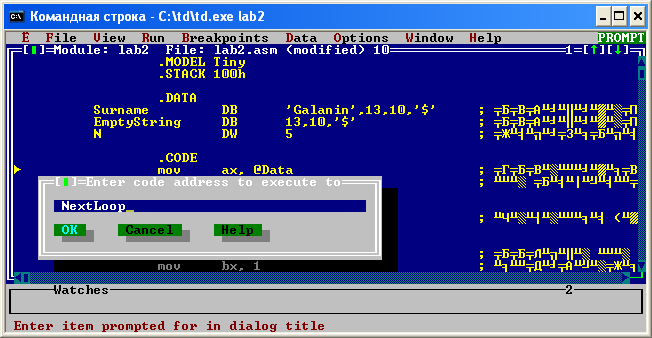
\includegraphics[width=.99\linewidth]
            {../_INCLUDES/task-4-9/td-Alt-F9.png}
        \caption{\textbf{Alt} + \textbf{F9}}
        \label{fig:task_4_9__Alt_F9}
    \end{minipage}
    \begin {minipage}{0.32\textwidth}
        \centering
        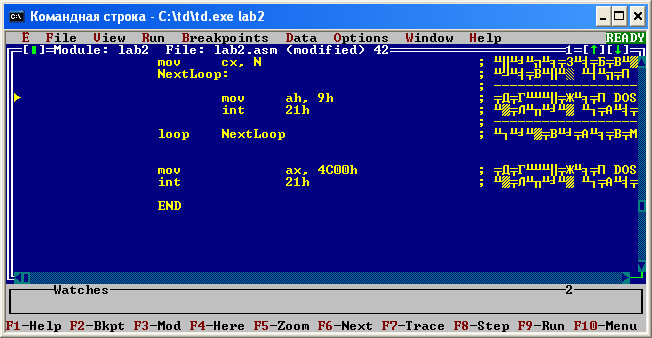
\includegraphics[width=.99\linewidth]
            {../_INCLUDES/task-4-9/td-Alt-F9-result.png}
        \caption{Переход к метке}
        \label{fig:task_4_9__Alt_F9_result}
    \end{minipage}
\end{figure}

Жмем \textbf{F10}. Жмем два раз \textbf{вправо}. Выбираем пункт \textbf{View}. Жмем 7 раз \textbf{вниз}. Выбираем пунт \textbf{CPU}. \textbf{Enter}. Результат на рисуноке~\ref{fig:task_4_9__td_View_CPU} (стр.~\pageref{fig:task_4_9__td_View_CPU}).

\begin{figure}[!htp]
    \centering
    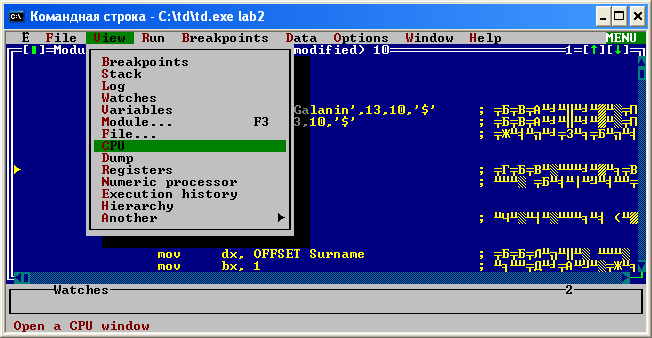
\includegraphics[width=8cm]
        {../_INCLUDES/task-4-9/td-View-CPU.png}
    \caption{}
    \label{fig:task_4_9__td_View_CPU}
\end{figure}

\begin{figure}[!htp]
    \centering
    \begin{minipage}{0.32\textwidth}
        \centering
        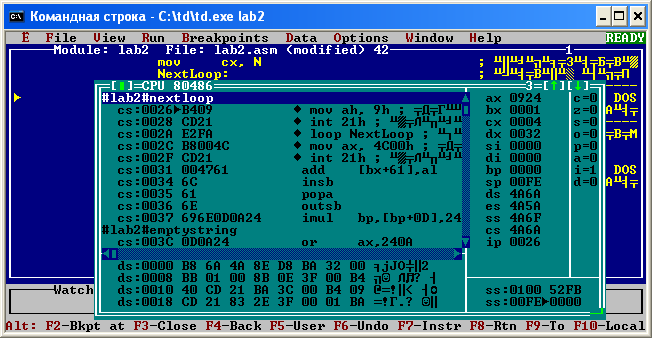
\includegraphics[width=.99\linewidth]
            {../_INCLUDES/task-4-9/0.png}
        \caption{0 Шаг}
        \label{fig:task_4_9}
    \end{minipage}
    \begin {minipage}{0.32\textwidth}
        \centering
        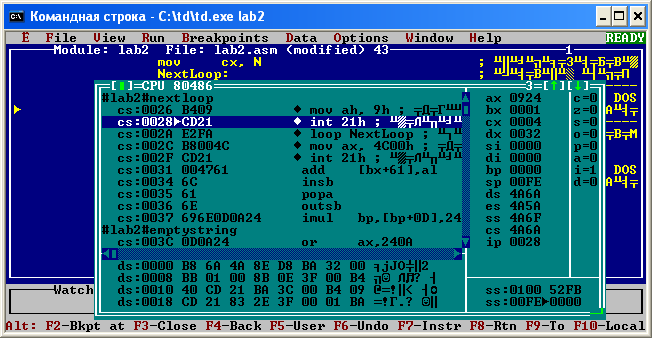
\includegraphics[width=.99\linewidth]
            {../_INCLUDES/task-4-9/1.png}
        \caption{1) \textbf{F7}}
        \label{fig:task_4_9}
    \end{minipage}
    \begin {minipage}{0.32\textwidth}
        \centering
        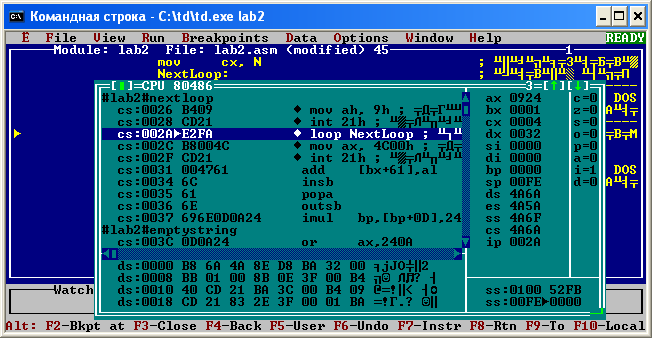
\includegraphics[width=.99\linewidth]
            {../_INCLUDES/task-4-9/2.png}
        \caption{2) \textbf{F7}}
        \label{fig:task_4_9}
    \end{minipage}
\end{figure}

\begin{figure}[!htp]
    \centering
    \begin{minipage}{0.32\textwidth}
        \centering
        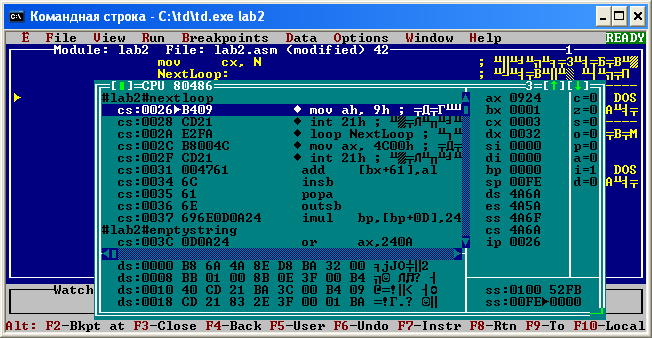
\includegraphics[width=.99\linewidth]
            {../_INCLUDES/task-4-9/3.png}
        \caption{3) \textbf{F7}}
        \label{fig:task_4_9}
    \end{minipage}
    \begin {minipage}{0.32\textwidth}
        \centering
        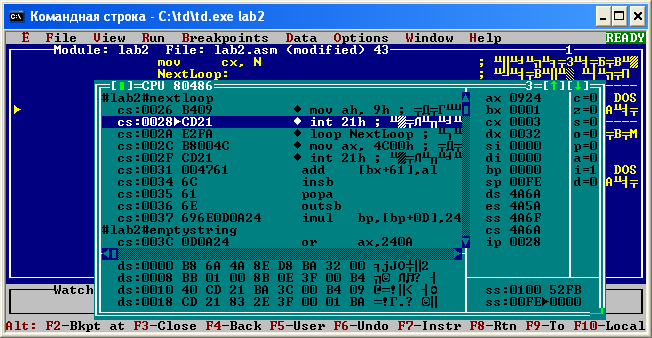
\includegraphics[width=.99\linewidth]
            {../_INCLUDES/task-4-9/4.png}
        \caption{4) \textbf{F7}}
        \label{fig:task_4_9}
    \end{minipage}
    \begin {minipage}{0.32\textwidth}
        \centering
        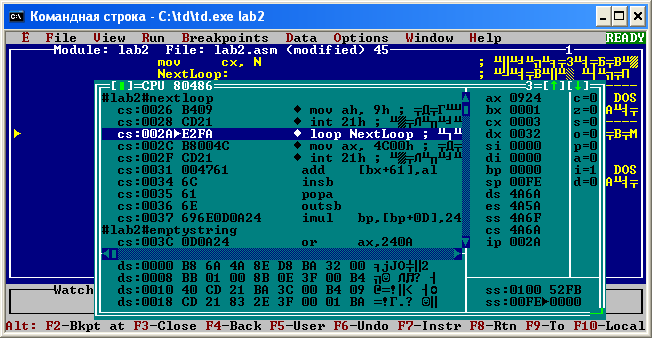
\includegraphics[width=.99\linewidth]
            {../_INCLUDES/task-4-9/5.png}
        \caption{5) \textbf{F7}}
        \label{fig:task_4_9}
    \end{minipage}
\end{figure}

\begin{figure}[!htp]
    \centering
    \begin{minipage}{0.32\textwidth}
        \centering
        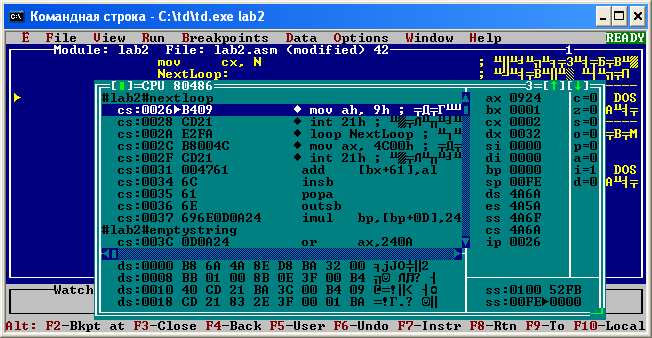
\includegraphics[width=.99\linewidth]
            {../_INCLUDES/task-4-9/6.png}
        \caption{6) \textbf{F7}}
        \label{fig:task_4_9}
    \end{minipage}
    \begin {minipage}{0.32\textwidth}
        \centering
        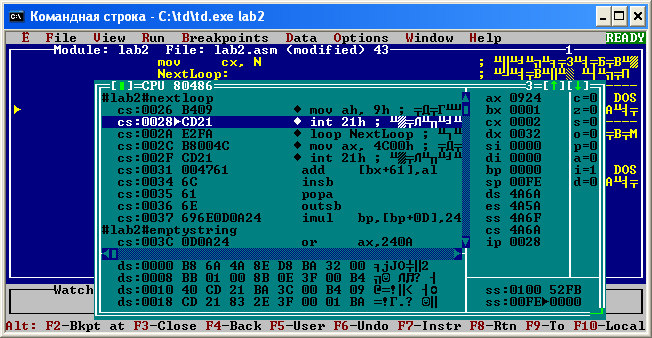
\includegraphics[width=.99\linewidth]
            {../_INCLUDES/task-4-9/7.png}
        \caption{7) \textbf{F7}}
        \label{fig:task_4_9}
    \end{minipage}
    \begin {minipage}{0.32\textwidth}
        \centering
        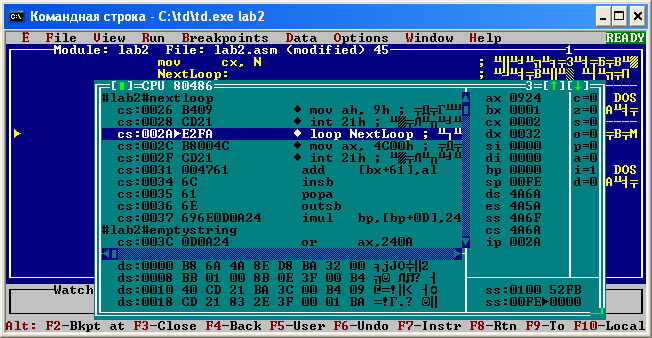
\includegraphics[width=.99\linewidth]
            {../_INCLUDES/task-4-9/8.png}
        \caption{8) \textbf{F7}}
        \label{fig:task_4_9}
    \end{minipage}
\end{figure}

\begin{figure}[!htp]
    \centering
    \begin{minipage}{0.32\textwidth}
        \centering
        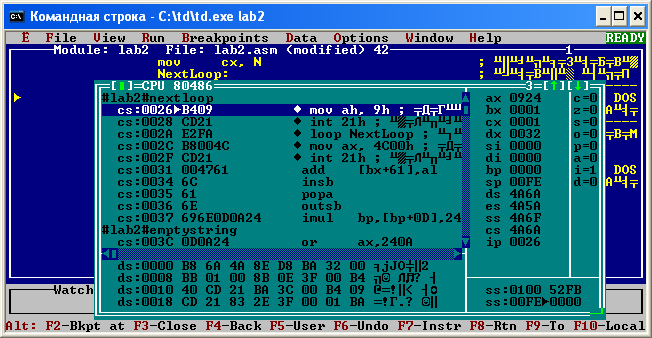
\includegraphics[width=.99\linewidth]
            {../_INCLUDES/task-4-9/9.png}
        \caption{9) \textbf{F7}}
        \label{fig:task_4_9}
    \end{minipage}
    \begin {minipage}{0.32\textwidth}
        \centering
        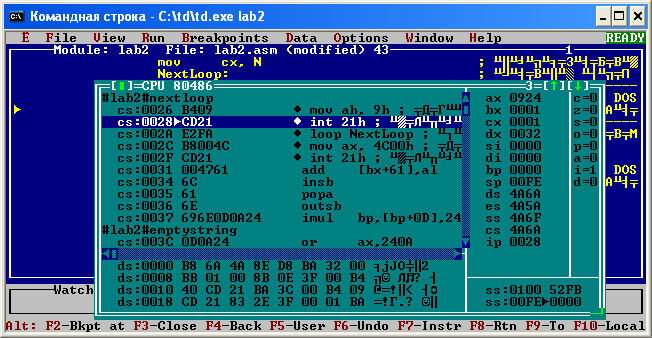
\includegraphics[width=.99\linewidth]
            {../_INCLUDES/task-4-9/10.png}
        \caption{10) \textbf{F7}}
        \label{fig:task_4_9}
    \end{minipage}
    \begin {minipage}{0.32\textwidth}
        \centering
        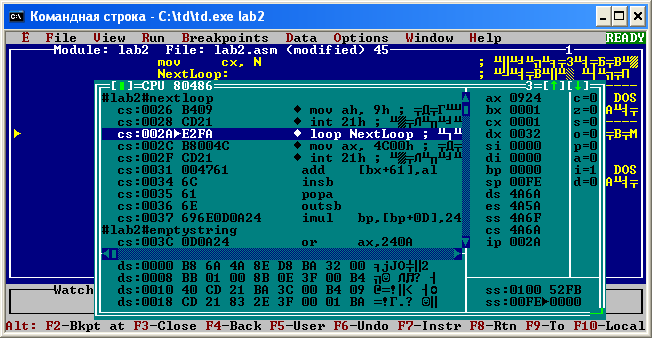
\includegraphics[width=.99\linewidth]
            {../_INCLUDES/task-4-9/11.png}
        \caption{11) \textbf{F7}}
        \label{fig:task_4_9}
    \end{minipage}
\end{figure}

\begin{figure}[!htp]
    \centering
    \begin{minipage}{0.32\textwidth}
        \centering
        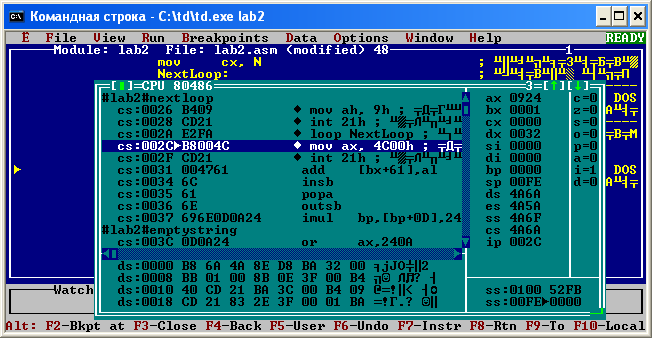
\includegraphics[width=.99\linewidth]
            {../_INCLUDES/task-4-9/12.png}
        \caption{12) \textbf{F7}}
        \label{fig:task_4_9}
    \end{minipage}
    \begin {minipage}{0.32\textwidth}
        \centering
        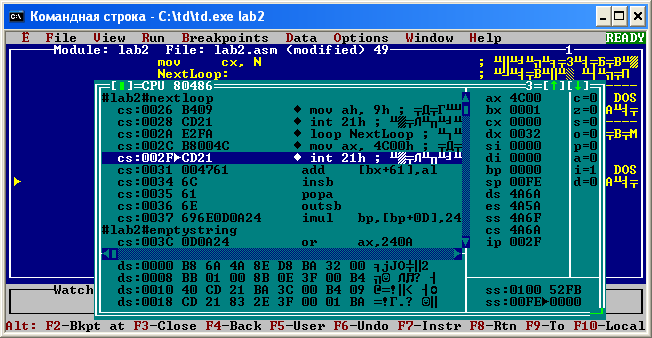
\includegraphics[width=.99\linewidth]
            {../_INCLUDES/task-4-9/13.png}
        \caption{13) \textbf{F7}}
        \label{fig:task_4_9}
    \end{minipage}
    \begin {minipage}{0.32\textwidth}
        \centering
        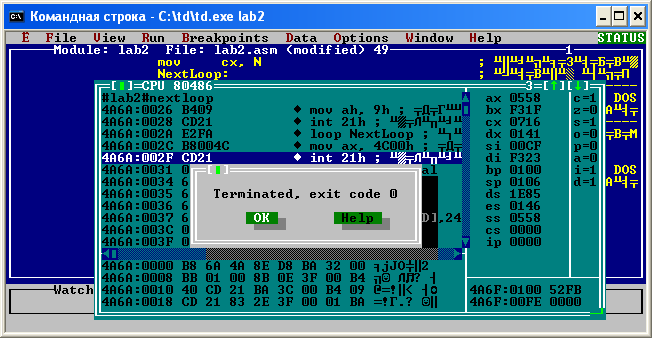
\includegraphics[width=.99\linewidth]
            {../_INCLUDES/task-4-9/14.png}
        \caption{14) \textbf{F7}}
        \label{fig:task_4_9}
    \end{minipage}
\end{figure}

Значение регистров после метки NextLoop с шагом \textbf{F7} в таблице~\ref{tab:task_4_9__table} (стр. \pageref{tab:task_4_9__table}).

\begin{table}[!htp]
    \centering
    \caption{Значения регистров после метки NextLoop с шагом \textbf{F7}}
    \label{tab:task_4_9__table}
    \begin{tabular}{|c|c|c|c|c|c|} 
        \hline
        № шага  & IP    & AX    & BX    & CX    & DX    \\ \hline
        \hline
        0       & 0026  & 0924  & 0001  & 0004  & 0032  \\ \hline
        1       & 0028  & 0924  & 0001  & 0004  & 0032  \\ \hline
        2       & 002A  & 0924  & 0001  & 0004  & 0032  \\ \hline
        3       & 0026  & 0924  & 0001  & 0003  & 0032  \\ \hline
        4       & 0028  & 0924  & 0001  & 0003  & 0032  \\ \hline
        5       & 002A  & 0924  & 0001  & 0003  & 0032  \\ \hline
        6       & 0026  & 0924  & 0001  & 0002  & 0032  \\ \hline
        7       & 0028  & 0924  & 0001  & 0002  & 0032  \\ \hline
        8       & 002A  & 0924  & 0001  & 0002  & 0032  \\ \hline
        9       & 0026  & 0924  & 0001  & 0001  & 0032  \\ \hline
        10      & 0028  & 0924  & 0001  & 0001  & 0032  \\ \hline
        11      & 002A  & 0924  & 0001  & 0001  & 0032  \\ \hline
        12      & 002C  & 0924  & 0001  & 0000  & 0032  \\ \hline
        13      & 002F  & 4c00  & 0001  & 0000  & 0032  \\ \hline
        14      & 0000  & 0558  & F31F  & 0716  & 0141  \\ \hline
    \end{tabular}
\end{table}

\newpage
